\documentclass[12pt] {article}
\usepackage{times}
\usepackage{setspace}
%\doublespacing
\usepackage[margin=0.7in,bottom=1in,top=0.1in]{geometry}
\usepackage{graphicx}



\begin{document}

\title{Quiz - ECS 275A}
\author{Ahmed H. Mahmoud}
\date{June 7th, 2017} 

\maketitle

\textbf{Q:} What is the meaning of a BSSRDF?

\textbf{A:} Bidirectional Scattering-Surface Reflectance Distribution Function (BSSRDF) is the generalization of the Bidirectional Reflectance Distribution Function (BRDF) which describes the light transport between any two rays that hit a surface, whereas the BRDF assumes the light entering a material leaves the material at the same position. The difference between BSSRDF and BRDF is shown in Figure \ref{fig:bssrdf}.
\newline

\begin{figure}[!tbh]
 \centering        
 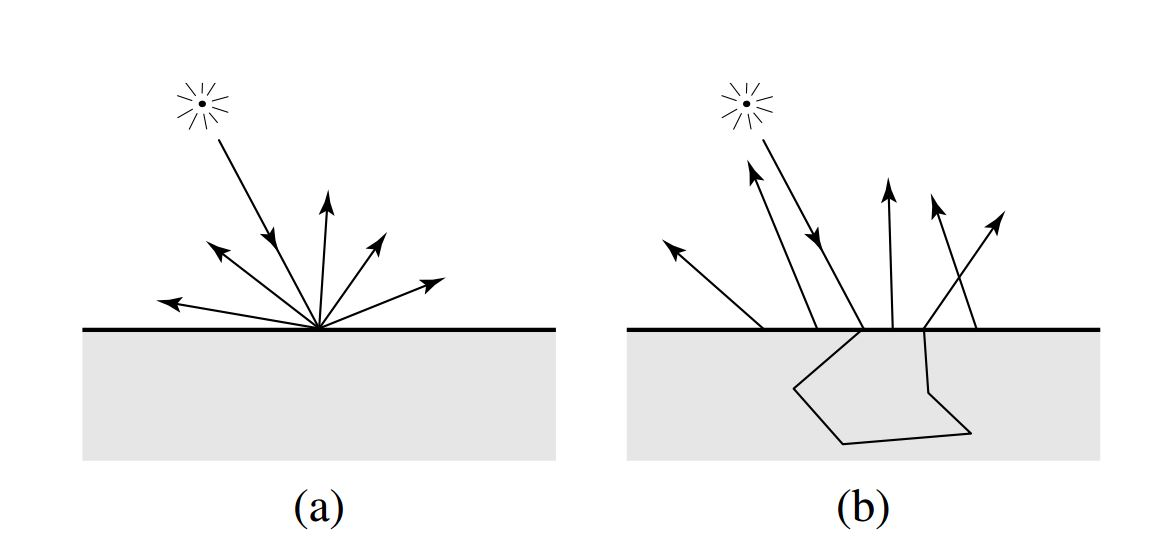
\includegraphics[width=0.6\textwidth]{BSSRDF.jpg}
     \caption{Scattering of light in (a) a BRDF, and (b) a BSSRDF}
   \label{fig:bssrdf}
\end{figure} 


\textbf{Q:} Suppose we need to sample a phase function $p(A, B)$ depending only on the angle theta between the unit vector $A$ for the incoming direction and $B$ for the scattering direction, for example, to do Monte Carlo light tracing in a participating medium. Given the vector $A$, how can we choose $B$ so that its probability density is $p(A, B)$.

\textbf{A:}
We start by calculating the inverse cumulative distribution function of $p(A,B)$. Then we generate a random variable $u$ over the interval $[0,1)$. The resulting sample $F^{-1}(u)$ matches the the phase/distribution function $p(A,B)$.


\end{document}
